\documentclass[10pt,fleqn]{article} % Default font size and left-justified equations
\usepackage[%
    pdftitle={Centrale Supelec 2018},
    pdfauthor={UPSTI}]{hyperref}

\input{style/new_style}
\input{style/macros_SII}
\usepackage{multicol}
\usepackage{siunitx}
%\usepackage{picins}
\fichetrue
%\fichefalse

\proftrue
\proffalse

\tdtrue
%\tdfalse

\courstrue
\coursfalse

% -------------------------------------
% Déclaration des titres
% -------------------------------------

\def\discipline{Sciences \\Industrielles de \\ l'Ingénieur}
\def\xxtete{Sciences Industrielles de l'Ingénieur}


\def\classe{\textsf{UPSTI}}
\def\xxnumpartie{CCS 2019}
\def\xxpartie{Chirurgie mini-invasive robotisée avec
stabilisation des mouvements physiologiques}

\def\xxnumchapitre{Concours Centrale Supelec}%Révision 1 \vspace{.2cm}}
\def\xxchapitre{PSI 2019}

\def\xxposongletx{2}
\def\xxposonglettext{1.45}
\def\xxposonglety{16}%16

\def\xxonglet{\textsf{CCS 2019}}

\def\xxactivite{TD 01}
\def\xxauteur{\textsl{UPSTI}}


\def\xxtitreexo{Chirurgie mini-invasive robotisée avec
stabilisation des mouvements physiologiques}
\def\xxsourceexo{\hspace{.2cm} \footnotesize{Concours Centrale Supelec PSI 2019}}

\def\xxcompetences{%
\textsl{%
%\textbf{Savoirs et compétences :}\\
}}

\def\xxfigures{
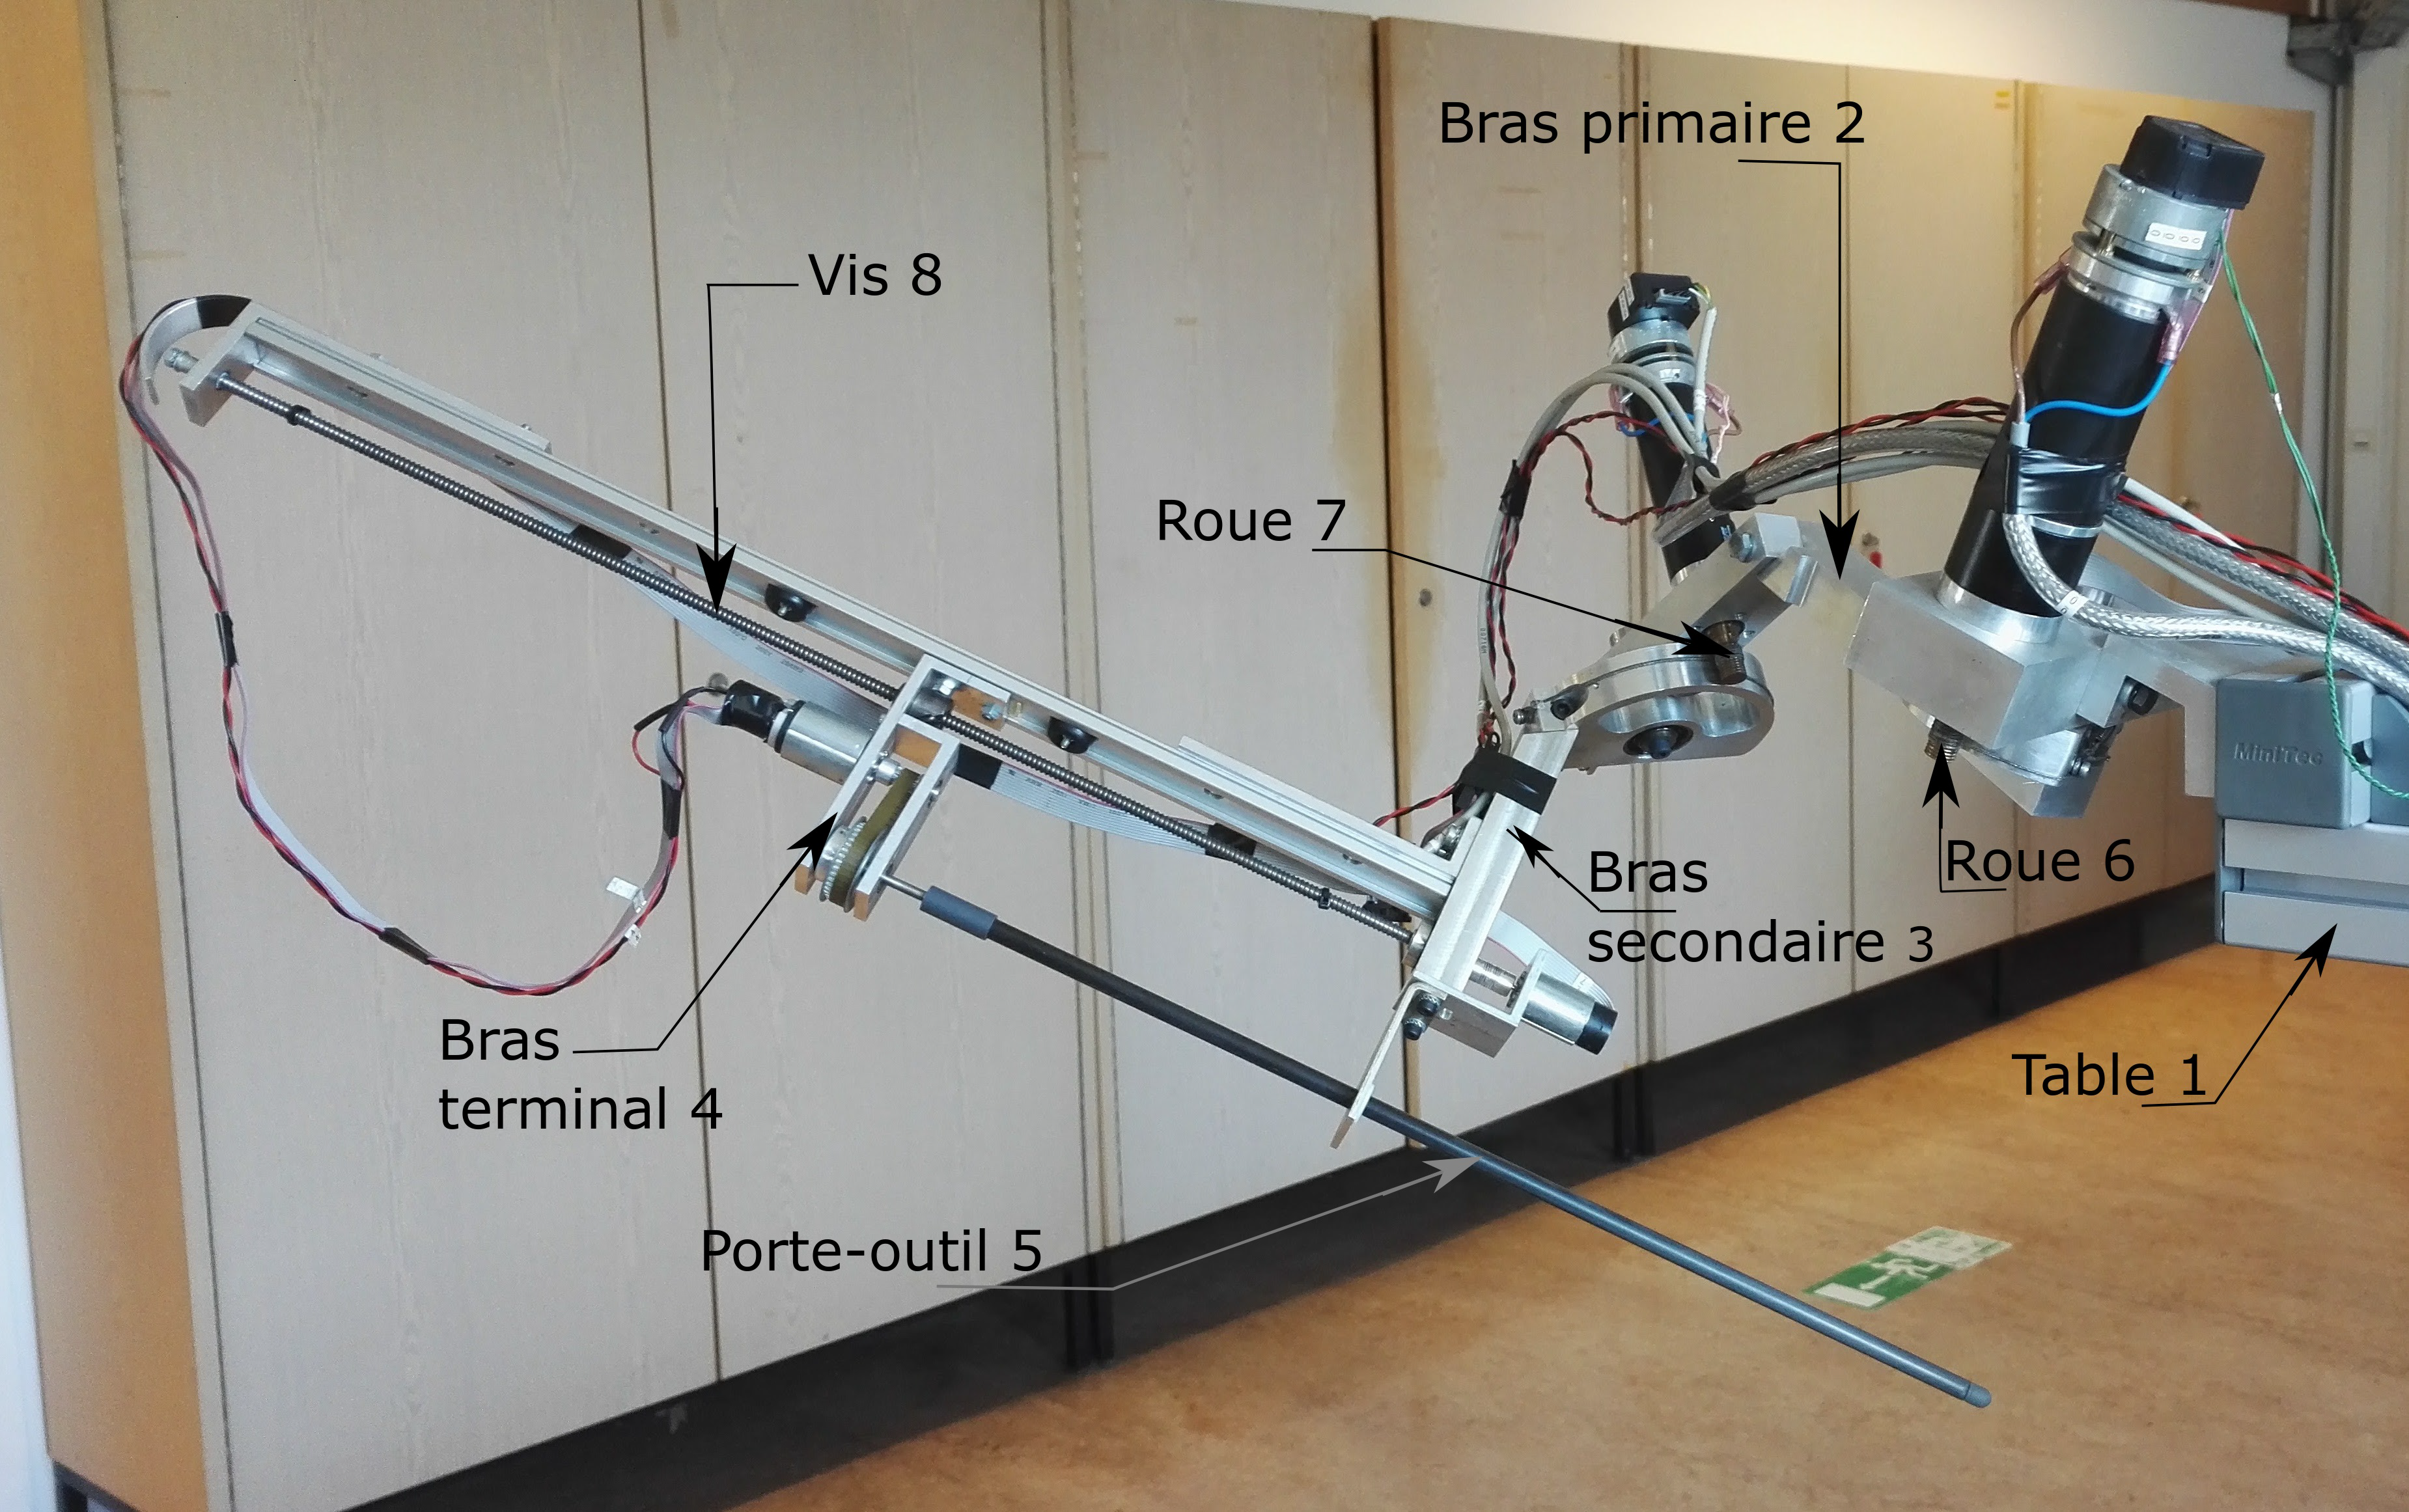
\includegraphics[width=.55\textwidth]{images/fig_00}
}%figues de la page de garde

\def\xxpied{%
Chirurgie mini-invasive robotisée\\
Concours Centrale Supelec -- PSI 2019%
}

\setcounter{secnumdepth}{5}
%---------------------------------------------------------------------------

\usepackage{bm}
\begin{document}
%\chapterimage{png/Fond_Cin}
\input{style/new_pagegarde}
\vspace{4.5cm}
\pagestyle{fancy}
\thispagestyle{plain}


\def\columnseprulecolor{\color{ocre}}
\setlength{\columnseprule}{0.4pt} 

\section{Analyse des propriétés des signaux physiologiques}

\begin{obj}
Analyser les propriétés des signaux physiologiques et en déduire des éléments du cahier des charges
de la loi de commande pour assurer le déplacement du robot avec le niveau de précision requis.
\end{obj}

\subsection{Analyse des propriétés des signaux des mouvements physiologiques}

\begin{obj}
Proposer un algorithme permettant de mettre en évidence les propriétés des mouvements respiratoires.
\end{obj}
\subparagraph{}
En première approximation, on peut dire que ce signal est périodique, de période \SI{4,8}{s}. La valeur maximale est de \SI{5}{mm} et la valeur minimale est de \SI{-2,5}{s}.
Si on avait à la modéliser par un signal sinusoïdal on aurait $e(t)=3,75 \sin\dfrac{2\pi}{4,8} t + 1,25$.

\subparagraph{}
D'après la définition, 
$\hat{S}\left( f_n\right)= \dfrac{1}{N_f} \sum \limits_{k=0}^{N_f-1} s\left[kT_e\right] \text{e}^{-i 2 \pi f_nT_e k}$

$= \dfrac{1}{N_f} \left(
 s\left[0 T_e\right] \text{e}^{-i 2 \pi f_nT_e 0} + 
 s\left[T_e\right] \text{e}^{-i 2 \pi f_nT_e } + ... 
 s\left[\left( N_f-1\right)T_e\right] \text{e}^{-i 2 \pi f_nT_e \left( N_f-1\right)}\right)$

$= \dfrac{1}{N_f} \left(
 s\left[0\right] + 
 s\left[T_e\right] \text{e}^{-i 2 \pi f_nT_e } + ... 
 s\left[\left( N_f-1\right)T_e\right] \text{e}^{-i 2 \pi f_nT_e \left( N_f-1\right)}\right)$.
 
 On a donc $l_k\left(f_n\right)=\dfrac{1}{N_f}\text{e}^{-i 2 \pi f_nT_e k}$.
 
\end{document}




\subparagraph{}\textit{}


\begin{center}
\includegraphics[width=\linewidth]{images/img_04}
%\textit{}
\end{center}



